%\documentclass[a4paper,twoside,12pt]{book}
\documentclass[twoside, openright, 11pt]{report}
\usepackage[spanish]{babel}
\usepackage[utf8]{inputenc}
\usepackage{graphicx} %Para poder insertar las imagenes
\usepackage{float}
\usepackage{listings}
\usepackage{xcolor}
\usepackage[hidelinks]{hyperref}   % optional, nicer for clickable links
\usepackage{geometry} % <-- añadir para ajustar márgenes temporalmente
%\usepackage{url}
%\usepackage{blindtext}

\begin{document}

\begin{titlepage}


\newlength{\centeroffset}
\setlength{\centeroffset}{-0.5\oddsidemargin}
\addtolength{\centeroffset}{0.5\evensidemargin}
\thispagestyle{empty}

\noindent\hspace*{\centeroffset}\begin{minipage}{\textwidth}

\centering

\includegraphics[width=0.9\textwidth]{imagenes/logo_ugr}\\[1.4cm]

\textsc{ \Large TRABAJO FIN DE GRADO\\[0.2cm]}
\textsc{ GRADO DE INGENIERÍA EN INFORMÁTICA}\\[1cm]
% Upper part of the page
%
% Title
{\huge\bfseries NutriPlan\\
}
\noindent\rule[-1ex]{\textwidth}{3pt}\\[3.5ex]
{\large\bfseries Aplicación para la Gestión de Recetas}
\end{minipage}

\vspace{0.5cm}
\noindent\hspace*{\centeroffset}\begin{minipage}{\textwidth}
\centering

\textbf{Autor}\\ {Aissa Rouk El Masoudi}\\[2.5ex]
\textbf{Directores}\\
{CARLOS RODRIGUEZ DOMINGUEZ}\\[2cm]

\includegraphics[width=0.3\textwidth]{imagenes/logo-ceuta.jpg}\\[0.1cm]
\textsc{Facultad de Educación, Tecnología y Economía de Ceuta}\\
\textsc{---}\\
Granada, 15 de Junio de 2025
\end{minipage}
\end{titlepage}
\let\cleardoublepage\clearpage

\chapter*{}
\begin{flushright}
\textit{Dedicado a \\
...}
\end{flushright}
\thispagestyle{empty}

\lstdefinelanguage{TypeScript}{
	keywords={typeof, new, true, false, catch, function, return, null, catch, switch, var, if, in, while, do, else, case, break, export, type, string, number, boolean, interface, extends, implements, import, from, as},
	keywordstyle=\color{blue}\bfseries,
	ndkeywords={class, export, boolean, throw, implements, import, this},
	ndkeywordstyle=\color{teal}\bfseries,
	identifierstyle=\color{black},
	sensitive=true,
	comment=[l]{//},
	morecomment=[s]{/*}{*/},
	commentstyle=\color{gray}\ttfamily,
	stringstyle=\color{green!50!black}\ttfamily,
	morestring=[b]',
	morestring=[b]"
}

\lstset{
	language=TypeScript,
	basicstyle=\ttfamily\small,
	backgroundcolor=\color{gray!10},
	frame=single,
	showstringspaces=false,
	breaklines=true,
	framextopmargin=5pt,
	framexbottommargin=5pt,
	framexrightmargin=5pt,
	columns=fullflexible,
	tabsize=1,
}


\chapter*{Resumen} % si no queremos que añada la palabra "Capitulo"
\addcontentsline{toc}{chapter}{Resumen} % si queremos que aparezca en el índice
\markboth{RESUMEN}{RESUMEN} % encabezado
\thispagestyle{empty}
OMS cita que en 2022 el 43\% de los adultos en el mundo tenía sobrepeso, y el 16\% padecía obesidad, lo que equivale a unos 890 millones de adultos obesos\cite{OMSObesidadySobrepeso}. Desde 1990, el número de personas con obesidad se han más que duplicado entre los adultos y se han cuadruplicado entre los adolescentes\cite{ONUAAComercioAlimentosyObesidad}.
\\Esta situación afecta a personas de todas las edades, regiones y tiene graves consecuencias para la salud, economía y los sistemas sanitarios, hace cada vez más urgente fomentar hábitos alimentarios saludables y estrategias que promuevan una alimentación consciente, eficiente y sostenible.
\\De este contexto surge NutriPlan, una aplicación de Meal Planning y gestión de recetas cuyo objetivo es fomentar un estilo de vida saludable, económico y sostenible, reduciendo el desperdicio de alimentos. 
Esta idea surgió en mi experiencia como estudiante Erasmus, dónde descubrí que al realizar la lista de la compra manualmente y verificar cuáles ingredientes tenía, se ahorraba más dinero en la compra, desperdiciaba menos comida y lo más importante, comía sano.

\chapter*{Abstract} % si no queremos que añada la palabra "Capitulo"
\addcontentsline{toc}{chapter}{Abstract} % si queremos que aparezca en el índice
\markboth{ABSTRACT}{ABSTRACT} % encabezado
\thispagestyle{empty}
This project will proceed with the design and development of a recipe application...

\tableofcontents % indice de contenidos

\cleardoublepage
\addcontentsline{toc}{chapter}{Lista de figuras} % para que aparezca en el indice de contenidos
\listoffigures % indice de figuras

\cleardoublepage
\addcontentsline{toc}{chapter}{Lista de tablas} % para que aparezca en el indice de contenidos
\listoftables % indice de tablas

\chapter{Introducción}\label{cap.introduccion}
  \section{Motivación} 
  Siempre quise crear algo relacionado con mis dos vocaciones, ayudar a las personas y la programación, cada vez que tengo un momento libre intento utilizarlo para pensar cómo hacer el mundo un sitio mejor, qué ideas de aplicaciones podrían aportar algo a las necesidades de la sociedad, esto me llevó a crear varias aplicaciones desde crear una aplicación de escritura reflexiva para mejora personal, hasta la creación de un software administrador de tareas.
  \\
  Esta idea de proyecto surgió cuando estaba en un programa de movilidad estudiantil, después de varios meses realizando la compra e intentando reducir su gasto sin que baje la calidad de mi dieta, noté al principio que cuando realizaba una lista de la compra, gastaba mucho menos de lo que debía, porque no compraba cosas innecesarias o duplicadas. Al cabo de otro tiempo, descubrí que si realizaba mi plan dietético de manera específica antes de realizar la compra semanal, este gasto era mucho menor porque en la lista añadía las cantidades de cada ingrediente que necesitaba, esto no solo redujo mis compras innecesarias, sino que me motivaba a comprar las cantidades exactas necesarias de cada producto o ingrediente, reduciendo el coste de mi compra semanal. 
  \\
  Además de este beneficio económico, percibí que la realización de esta práctica me impulsaba a respetar las cantidades planificadas en mi dieta, haciendo que, esta no solo se volviera más saludable, sino también más variada.
  La Librería Nacional de Medicina Estadounidense realizó un estudio dónde se concluyó que \textit{“la planificación dietética está asociada a una dieta más saludable y una menor prevalencia de obesidad”}\cite{NLMMealPlanningBenefits}, y que \textit{“la práctica de esta podría ser potencialmente relevante para la prevención de la obesidad”}\cite{NLMMealPlanningBenefits}. 
  \\
  Una publicación de la Comisión Europea afirma que los hogares generan más de la mitad del desperdicio alimentario existente y que una de sus causas es la insuficiente planificación de las compras y de las comidas, lo que no solo perjudica la economía familiar, sino que también tiene un impacto ambiental significativo.
  \\
  Todo esto me llevó a crear NutriPlan, una aplicación que satisface todas estas necesidades. Un software que ayuda a los usuarios mediante la creación de una lista de la compra con las recetas ya registradas por el usuario, lleva un seguimiento de su despensa recordando que ingredientes aún tiene disponibles, y calculando cuándo cada ingrediente que se acaba.
  
  \section{Objetivos} 
  El objetivo de este proyecto es la creación de una aplicación móvil que facilite la planificación dietética, haciéndola más sencilla y eficiente promoviendo todos los beneficios discutidos anteriormente en la motivación; lleve un seguimiento de la despensa del usuario y modifique esta cada vez que se realice la compra, planificación de la dieta semanal mediante la adición o eliminación de ingredientes en la despensa.
  \\
  \\
  El resultado será una aplicación con las siguientes funcionalidades:
  
  
  \begin{itemize}
  	\item Gestión de recetas
  	\begin{itemize}
  		\item Adición de una nueva receta mediante la introducción del nombre, enlace, tiempo de preparación y la cantidad de porciones de la receta; la adición de los ingredientes correspondientes a la receta.
  		\item Eliminación o edición de una receta ya existente.
  	\end{itemize}
  	
  	\item Gestión de ingredientes
  	\begin{itemize}
  		\item Adición de nuevos ingredientes a una receta con sus cantidades.
  		\item Posibilidad de buscar (mediante un motor de búsqueda) ingredientes nuevos para añadirlos a una receta que se esté creando.
  	\end{itemize}
  	
  	\item Gestión de dieta semanal
  	\begin{itemize}
  		\item El usuario podrá asignar una o varias recetas para cada comida del día (desayuno, comida, cena), esta asignación es modificable.
  	\end{itemize}
  	
  	\item Gestión de la lista de la compra
  	\begin{itemize}
  		\item El programa será el encargado de la creación de una lista de la compra. Esto se realizará sumando las cantidades de los ingredientes similares de todas las recetas y restando a esta suma las cantidades que haya en la despensa.
  	\end{itemize}
  \end{itemize}
  
  \section{Estructura de la memoria}
  %Explicar de qué va la memoria capítulo por capítulo brevemente
  
  \section{Recursos utilizados}
  
  \section{Planificación temporal}
  

\chapter{Estado del arte}\label{cap.estado del arte}
	\section{Fundamentos}
		\subsection*{La planificación dietética o Meal prepping}
		Hoy en día es difícil tener un estilo de vida saludable dada la falta de tiempo que causan las responsabilidades como el trabajo, familia, sueño, etc; varios datos muestran que los jóvenes consumen mucha menos fruta y verdura de la cantidad recomendada diaria, y que estos consumen mucho más comida basura de la que se recomienda \cite{NLMDifficultyEatingHealthy}.
		\\
		Otro análisis indica que la mayor barrera que impide a las personas de seguir una dieta saludable es la falta de tiempo, el no querer abandonar alimentos favoritos y los elevados precios de las comidas sanas \cite{NLMDifficultyEatingHealthy}. A mucha gente le cuesta mantener ese balance entre trabajar y tener una vida sana y he de ahí donde surge la planificación de dietas o meal planning, una práctica que consiste en planificar las comidas de un periodo futuro determinado (generalmente una semana). La mayor parte de las personas planifican tres comidas por día para los días laborales (de lunes a viernes), pero esta práctica es completamente personalizable.\cite{HowToMealPrep}.
		\\
		\\
		El método de uso de esta práctica puede variar dependiendo de la persona, pero la metodología más común es la siguiente.
		%
		% Pasos para crear una lista de la compra
		%
		\begin{enumerate}
			\item Se elabora una tabla en la que se escriben todos los días de la semana en las columnas y los tipos de comida (desayuno, comida, cena, y en su caso merienda o aperitivo) en las filas  (Figura~\ref{fig:Plantillamealplan}). En cada celda se anotan las recetas o alimentos que se consumirán en el día y la comida correspondiente. A pesar de que este proceso se puede realizar en papel, resulta preferible hacerlo en un ordenador ya que facilita la edición y corrección de posibles errores. La tabla resultante será similar a la de la Figura~\ref{fig:Plantillamealplanrellenada}.
			
			\begin{figure}[H]
				\centering
				\includegraphics[width=1\textwidth]{./imagenes/PlantillaTablamealPlanning.png}
				\caption{Plantilla planificación de comidas}
				\label{fig:Plantillamealplan}
			\end{figure}
			
			\begin{figure}[H]
				\centering
				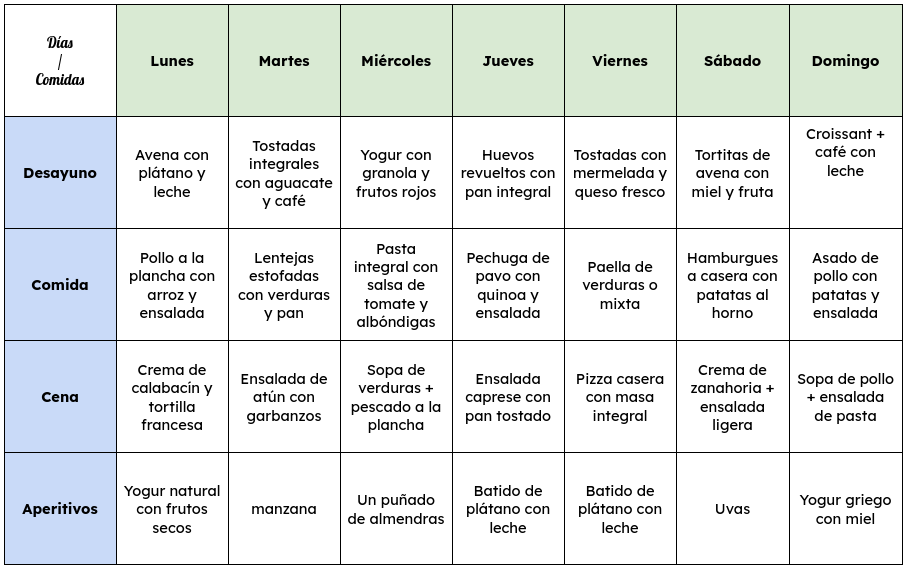
\includegraphics[width=1\textwidth]{./imagenes/PlantillaMealPlanningRellenada.png}
				\caption{Plantilla planificación de comidas}
				\label{fig:Plantillamealplanrellenada}
			\end{figure}
			
			\item Una vez completada la tabla con las recetas de la semana, se procede a listar los ingredientes necesarios para su preparación, incluyendo las cantidades específicas de cada uno (ver Tablas ~\ref{fig:TablaDeIngredientes} y ~\ref{fig:TablaCombinada}).
			
			\begin{table}[H]
				\centering
				\caption{Ejemplo de recetas con ingredientes comunes}
				\begin{tabular}{|p{3.5cm}|p{7cm}|p{3cm}|}
					\hline
					\textbf{Receta} & \textbf{Ingredientes} & \textbf{Cantidad (para 2 personas)} \\ \hline
					Pollo a la plancha con arroz y ensalada &
					Pechugas de pollo, arroz, lechuga, tomate, aceite de oliva, sal, pimienta, limón &
					Pollo 300 g; Arroz 120 g; Lechuga 100 g; Tomate 100 g; Aceite 10 ml \\ \hline
					
					Asado de pollo con patatas y verduras &
					Pollo, patatas, zanahoria, cebolla, aceite de oliva, sal, pimienta &
					Pollo 500 g; Patatas 400 g; Zanahoria 200 g; Cebolla 100 g; Aceite 20 ml \\ \hline
				\end{tabular}
				\label{fig:TablaDeIngredientes}
			\end{table}
			\begin{table}[H]
				\centering
				\caption{Lista de la compra combinada (optimizada)}
				
				\begin{tabular}{|p{5cm}|p{3cm}|}
					\hline
					\textbf{Ingredientes} & \textbf{Cantidad total} \\ \hline
					Pollo & 800 g \\ \hline
					Arroz & 120 g \\ \hline
					Lechuga & 100 g \\ \hline
					Tomate & 100 g \\ \hline
					Patatas & 400 g \\ \hline
					Zanahoria & 200 g \\ \hline
					Cebolla & 100 g \\ \hline
					Aceite de oliva & 30 ml \\ \hline
					Condimentos (sal, pimienta, romero, limón) & Al gusto \\ \hline
				\end{tabular}
			\label{fig:TablaCombinada}
			\end{table}
			
			\item Al obtener la lista de ingredientes necesarios para preparar las recetas planificadas, se revisan los productos disponibles (en el caso de un usuario común, el hogar). Esto permite la identificación de ingredientes que ya se poseen, haciendo que se puedan eliminar de la lista y ajustar la cantidad de los que se tengan parcialmente, evitando compras innecesarias y reduciendo el desperdicio alimentario. En nuestro ejemplo se supondrá que la despensa tiene 500 gramos de pollo y 100 de arroz (Tabla~\ref{fig:TablaCalculoIngr}), dando a la tabla de ingredientes final (Tabla~\ref{fig:TablaIngrFinal}))
			
			% Tabla de ingredientes a comprar y en despensa
			\begin{table}[H]
				\label{fig:TablaCalculoIngr}
				\centering
				\caption{Proceso de cálculo de ingredientes según la despensa}
				\begin{tabular}{|p{3cm}|p{3cm}|p{3cm}|p{3cm}|}
					\hline
					\textbf{Ingredientes} & \textbf{Necesario} & \textbf{En despensa} & \textbf{A comprar} \\ \hline
					Pollo & 800 g & 500 g & 300 g \\ \hline
					Arroz & 120 g & 100 g & 20 g \\ \hline
					Lechuga & 100 g & 0 & 100 g \\ \hline
					Tomate & 100 g & 0 & 100 g \\ \hline
					Patatas & 400 g & 0 & 400 g \\ \hline
					Zanahoria & 200 g & 0 & 200 g \\ \hline
					Cebolla & 100 g & 0 & 100 g \\ \hline
					Aceite de oliva & 30 ml & 0 & 30 ml \\ \hline
					Condimentos & Al gusto & 0 & Al gusto \\ \hline
				\end{tabular}
			\end{table}
		
			% Tabla de ingredientes finales
			\begin{table}[H]
				\centering
				\label{fig:TablaIngrFinal}
				\caption{Lista de la compra final optimizada}
				\begin{tabular}{|p{5cm}|p{3cm}|}
					\hline
					\textbf{Ingredientes} & \textbf{Cantidad a comprar} \\ \hline
					Pollo & 300 g \\ \hline
					Arroz & 20 g \\ \hline
					Lechuga & 100 g \\ \hline
					Tomate & 100 g \\ \hline
					Patatas & 400 g \\ \hline
					Zanahoria & 200 g \\ \hline
					Cebolla & 100 g \\ \hline
					Aceite de oliva & 30 ml \\ \hline
					Condimentos (sal, pimienta, romero, limón) & Al gusto \\ \hline
				\end{tabular}
			\end{table}
		
			
			\item Ahora que se ha obtenido la lista definitiva, es recomendable revisar la lista para ver si falta o se ha duplicado algún ingrediente, este paso no es necesario, pero ayuda a prevenir fallos. Después de esto faltaría solo realizar la compra.
		\end{enumerate}
		%
		%
		En los últimos años la planificación dietética ha ganado popularidad gracias a diversos factores sociales y culturales. De entre ellos destacan el auge de las redes sociales y la creciente influencia del culturismo y el deporte en la vida cotidiana. Plataformas como Instagram, YouTube o TikTok han facilitado el acceso a información sobre estos tópicos, motivando a muchos a estructurar sus dietas de forma más consciente y personalizada. Esta tendencia se observa también en el ámbito deportivo, como por ejemplo en el culturismo, donde el \textit{meal planning} es una práctica habitual y está estrechamente ligada a la preparación física. Varios estudios recientes muestran que los practicantes del culturismo adoptan esta práctica como parte fundamental de su entrenamiento, y que su fuente de información principal son las redes sociales y la comunidad digital \cite{helms2019,masoga2021,benjamins2021}.
		\\
		Este fenómeno no solo se refleja en ámbitos deportivos como el culturismo, sino también en la población general. Una investigación francesa descubrió que el 57,4\% de los habitantes planifican sus comidas al menos de manera ocasional, lo que evidencia un interés extendido en esta práctica como parte de la vida diaria \cite{ducrot2017}. De manera similar, en los Estados Unidos se estima que alrededor del 37\% organizan sus comidas con uno o dos días de antelación, lo que muestra el aumento del uso de la programación de menús fuera del ámbito deportivo \cite{fmi2015}. Esta convergencia entre el impacto social de las plataformas digitales, las prácticas del culturismo y la creciente adopción de \textit{meal planning} en la población aporta una razón y contexto sólidos para el desarrollo de herramientas digitales como \textit{NutriPlan}, cuyo objetivo es facilitar la organización alimentaria de manera sencilla, eficiente y accesible.
		\\\\
		El mercado de aplicaciones de planificación dietética está en constante expansión. Durante 2024 su valor alcanzó los 2,21 millones de dólares y se proyecta que crecerá al valor de 5,53 millones en 2033 \cite{businessresearchinsights2024}. Esta expansión viene impulsada por las nuevas tendencias como la de integración de la inteligencia artificial para la personalización de menús, la incorporación de prácticas sostenibles y la creación de comunidades digitales en torno a la alimentación. Además, la pandemia Covid-19 aceleró esta adopción al fomentar la preparación de comidas en casa y la planificación de las compras. Si se añade a la perspectiva el informe a nivel global de McKinsey, donde se afirma que el 50\% de los consumidores prioriza una alimentación saludable y más del 70\% desea mejorar su dieta, se demuestra un gran interés en este tópico \cite{mckinsey2023}.
		\\\\
		Los beneficios que aporta la planificación dietética son los que generan el interés por este movimiento, caracterizada por la falta de tiempo para funciones básicas como el sueño, la práctica de deporte o la cocina. La organización de comidas no sólo asegura una ingesta calórica y nutricional adecuada, sino que también contribuye en diversos aspectos de la vida diaria.\\
		\textbf{Ahorro de tiempo.} Una de las principales dificultades para mantener hábitos alimenticios saludables es la falta de tiempo. Según análisis hechos por la Biblioteca Nacional de Medicina de EE. UU., esta práctica reduce las compras improvisadas durante la semana y el tiempo empleado en decidir qué cocinar cada día, mejorando la eficiencia y disminuyendo la improvisación.
		\\
		\textbf{Reducción del estrés.} El meal planning ayuda a disminuir la tensión y el estrés derivados de la indecisión diaria sobre qué comer. Muchas personas deciden qué cocinar o comer en momentos de fatiga o poca motivación, lo que les conduce a optar por opciones menos saludables. Disponer de un plan y de los ingredientes necesarios facilita la elección de comidas más equilibradas y reduce la carga mental asociada a esta tarea.
		\\
		\textbf{Mejora de la dieta.} Diversos estudios han demostrado que cocinar en casa con mayor frecuencia se asocia a un consumo menor de carbohidratos, azúcares y grasas \cite{johnshopkins2014}. Además, la planificación dietética incentiva a cumplir objetivos calóricos y nutricionales mediante la compra anticipada de ingredientes. La evidencia científica indica que esta práctica está relacionada con una mejor calidad de dieta y una menor prevalencia de obesidad, lo que la hace potencialmente relevante en estrategias de prevención \cite{ducrot2017}.
		\\
		\textbf{Ahorro económico.} El uso de una lista de la compra estructurada se asocia con una mayor calidad de la dieta y, al mismo tiempo, un gasto más eficiente, ya que evita la adquisición de productos innecesarios \cite{jneb2017}, haciendo que ésta práctica beneficie tanto a la salud como a la economía.
		\\
		\textbf{Reducción del desperdicio alimentario.} Más de 59 millones de toneladas de residuos alimentarios, con un valor estimado en 132 millones; son generados anualmente en la Unión Europea. Una de las principales causas identificadas es la falta de planificación en la compra de alimentos en los hogares \cite{europeancommission2020}. El \textit{meal planning} contribuye en la mitigación de este problema, al fomentar la compra de cantidades ajustadas a las necesidades reales.
	
	
	\section{Lógica de la aplicación}
		\subsection{Decisiones de diseño: estructura, clases y casos de uso}
		En esta sección se explica de forma explícita y concisa qué decisiones de diseño se adoptaron en la aplicación y por qué se tomó cada una de ellas.
		

		\subsection{Casos de uso}
		\label{sec:casos_de_uso}
		
		En esta sección se enumeran y justifican los casos de uso principales de la aplicación \textit{NutriPlan}. Cada caso de uso incluye la motivación para su inclusión en el sistema, la forma en que se materializó en la implementación (referencias a módulos y ficheros relevantes) y una discusión sobre alternativas de diseño que se valoraron durante el desarrollo, explicando por qué la solución adoptada resultó la más adecuada para los objetivos del proyecto.
		
		\subsubsection*{Criterio de selección de los casos de uso}
		Los casos de uso se seleccionaron atendiendo a los requisitos funcionales básicos y a las prioridades del proyecto: permitir al usuario planificar sus comidas semanalmente, gestionar recetas e ingredientes, mantener un inventario de despensa y obtener una lista de la compra optimizada. Se dio preferencia a casos que maximizaran el beneficio al usuario final y que fueran implementables con un coste razonable de desarrollo.
		
		\subsubsection{1. Registro e inicio de sesión}
		La mayoría de aplicaciones permiten al usuario a crear una cuenta, iniciar sesión y mantener esta activa en el dispositivo. Esto es esencial para la separación de datos entre diferentes cuentas desde recetas privadas, despensas e planificaciones.\\
		Para ello la manera más sencilla y eficiente de implementar este caso de uso es mediante la creación de las pantallas de inicio y registro de sesión (\textit{LoginScreen} e \textit{RegisterScreen}) que permitan al usuario registrarse e iniciar sesión y mantener la cuenta activa en su dispositivo.\\
		Su implementación es con Firebase que proporciona \textit{Firebase Auth} que permite controlar el inicio de sesión y la autenticación.\\
		Existen varias alternativas que satisfacerían estos casos de us como la autenticación mediante un backend propio (REST/API) o servicios como Auth0. Estos se descartaron por la sobrecarga operativa y de configuración; Firebase ofrece integración directa con React Native, SDKs maduros y un tiempo de puesta en marcha muy inferior, adecuado para un TFG cuyo objetivo es priorizar la funcionalidad de cara al usuario.
		
		\subsubsection{2. Gestión de recetas (CRUD)}
		El componente más importante de nuestra aplicación es la receta y como en cada lista, el usuario tiene el derecho de crear, editar, eliminar, programar y listar las recetas con sus ingredientes y metadatos.\\
		Para ello se ha creado una arquitectura en la base de datos que separa entidades, funciones CRUD que comunican con la base de datos; pantallas y modales que muestran y permiten la edición de estos
		
		\subsubsection{3. Búsqueda de ingredientes y selección rápida}
		Ofrecer una búsqueda rápida de ingredientes para añadir a recetas o planificaciones. Para ello se creó una barra de búsqueda y se usó \textit{mini-search} como motor de búsqueda. Una búsqueda rápida y disponible offline mejora notablemente la experiencia de creación de recetas. Indexar en cliente reduce latencia y dependencia de la red en tareas frecuentes.\\
		Hay alternativas como búsquedas remotas (consultas a Firestore, o un servicio externo) o usar Fuse.js. Se prefirió MiniSearch por su rendimiento y simplicidad cuando los volúmenes de datos son pequeños/medios; la búsqueda remota hubiera incrementado latencias y coste de lecturas.
		
		\subsubsection{4. Planificación semanal de comidas}
		Como lo usual en cada planificación de menús, se tiene que poder asignar recetas o ingredientes a días y comidas (desayuno/comida/cena) y visualizar la semana con las asignaciones.  
		Para la Implementación de este caso se usan vistas (\textit{View}) en \texttt{MainScreen} como orquestador, \texttt{HeaderComponent} para selección del día y servicios \texttt{weeklyMeals-db-services.ts} para conectar con Firebase.\\
		Centralizar la planificación en \texttt{MainScreen} permite ofrecer una vista de contexto (lista de recetas previstas, botones de acción) y mantener la interacción rápida mediante modales para planificar. Se diseñó la entidad \texttt{WeeklyMeal} con campos mínimos que permiten tanto enlazar a una receta como a un ingrediente suelto.  
		Alternativas: sistema de planificación basado en reglas (p. ej. sugerencias automáticas por variedad nutricional) o planificación mediante calendarios externos. Estas ideas quedaron fuera del alcance inicial por aumentar la complejidad; se mantienen como mejoras futuras.
		
		\subsubsection{5. Gestión de despensa (inventario)}
		Uno de los beneficios de esta aplicación es la característica de mantener un inventario local con los ingredientes disponibles, actualizarlos en cualquier momento y hacer el cálculo automático de los ingredientes necesarios después de restar los presentes.
		Para ello, la implementación de \texttt{PantryScreen}, \texttt{ingredientPantry-db-services.ts} y componentes de tarjeta (\texttt{PlannedIngredientCard}, \texttt{IngredientCard}) para la visualización y el cálculo de los ingredientes planificados.  
		La despensa es clave para calcular la lista de la compra optimizada; por ello se optó por un modelo sencillo (\texttt{PantryItem}) que almacena cantidad y unidad por usuario. Las operaciones de suma/resta se realizan en servicios para mantener lógica centralizada, otras alternativas serían la sincronización exclusiva con supermercado (APIs externas) o almacenamiento solo en servidor. Se optó por persistencia con Firestore y caching local para permitir uso offline y reducir latencias.
		
		\subsubsection{6. Generación y gestión de la lista de la compra}
		Calcular la cantidad a comprar sumando ingredientes planificados y restando existencias en la despensa; marcar artículos como comprados.\\
		Implementación mediante la creación de \texttt{GroceryListScreen} para la muestra de los ingredientes a comprar, \texttt{groceryBought-db-services.ts} para la conexión con Firebase y \texttt{GroceryItem} que determina la estructura de los datos.
		Automatizar el cálculo de la lista de la compra es el valor diferencial central del producto. Al implementar este cálculo en la capa de servicios se asegura consistencia y evita duplicación de lógica en la UI. Marcar como comprado actualiza la despensa mediante operaciones atómicas o lotes para evitar desajustes.  
		Se podía haber delegado el cálculo en un backend propio o en funciones serverless para mayor control. Se valoró, pero se priorizó la simplicidad operativa aprovechando Firestore y la capacidad de operaciones por lotes en clientes.
		
		\subsubsection{7. Gestión de imágenes y multimedia}
		Descripción: permitir asociar imágenes a recetas y gestionar permisos de cámara/galería.  
		Implementación: subida a Firebase Storage y almacenamiento de \texttt{imageUrl} en documentos de receta; componentes que usan \texttt{react-native-image-picker}.  
		Justificación: imágenes mejoran la usabilidad y ayudan al reconocimiento visual de recetas; Firebase Storage facilita el almacenamiento y entrega CDN‑like.  
		Alternativas: almacenar imágenes como base64 en documentos o usar servicios externos de CDN; se descartaron por coste y complejidad de integración.
		
		\subsubsection*{Resumen y coherencia de los casos de uso}
		Los casos de uso seleccionados cubren el flujo completo esperado por el usuario: registrar y acceder a su cuenta, crear y organizar recetas, planificar menús, verificar la despensa y generar la lista de la compra. Cada caso se implementó priorizando latencia baja, disponibilidad offline y simplicidad de mantenimiento: decisiones que se reflejan en la estructura de ficheros (\texttt{src/Services/}, \texttt{src/Screens/}, \texttt{src/Components/}) y en el modelado de datos (\texttt{src/Types/Types.tsx}). Las alternativas más complejas (backend propio, normalización extrema, trazabilidad con Redux) se consideraron pero se descartaron por coste de desarrollo o por no aportar suficiente ventaja en la fase inicial del proyecto. Estas decisiones dejan, no obstante, margen para futuras migraciones y escalado cuando los requisitos lo exijan.

		
		\clearpage
		\newgeometry{left=0cm,right=0cm,top=5cm,bottom=0cm} 
		\thispagestyle{empty}
		\noindent
		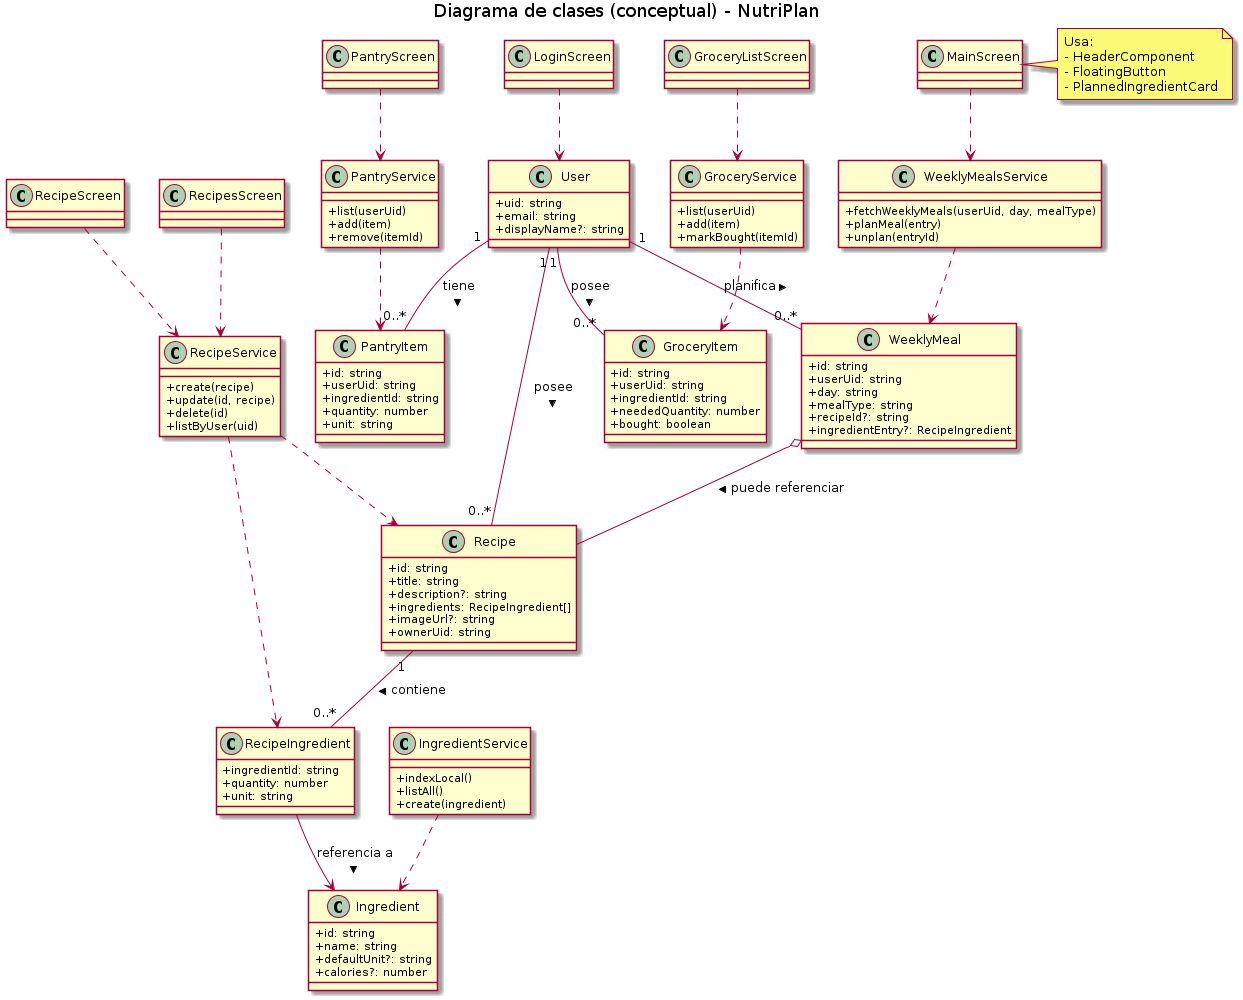
\includegraphics[width=\paperwidth,height=\paperheight,keepaspectratio]{imagenes/class_diagram}
		\clearpage
		\restoregeometry
		
		
		
		\subsection{Justificación del diagrama de clases y decisiones de diseño}
		\label{sec:justificacion_diagrama}
		
		En este apartado se justifican las decisiones que motivaron la separación representada en el diagrama de clases conceptual y se explica por qué cada componente, clase y relación fue diseñada de la manera mostrada.
		
		\paragraph{Criterio general de separación}
		La arquitectura sigue un principio de separación por responsabilidades (single responsibility, bajo acoplamiento y alta cohesión). Se decidió distinguir claramente entre:
		\begin{itemize}
			\item Entidades del dominio llamadas tipos en \textit{TypeScript} que son similares a las clases (tipos que modelan los datos): representan la forma y semántica de los objetos (User, Recipe, Ingredient, RecipeIngredient, WeeklyMeal, PantryItem, GroceryItem).
			\item Servicios por dominio (capa Services): encapsulan la lógica de persistencia y las operaciones con la base de datos de Firebase.
			\item Vistas/controladores (Pantallas y Componentes): orquestan flujos de interacción y presentan datos al usuario.
			\item Contexto y tipado (Context / Types): comparten estado global y contratos tipados entre capas.
		\end{itemize}
		Esta separación permite modificar la fuente de datos (por ejemplo migrar Firebase por otro BaaS) sin cambiar la UI, facilita la escritura de pruebas unitarias y simplifica la localización de la lógica de negocio.
		
		\paragraph{Entidades del dominio: elección de atributos}
		Las entidades modeladas en \texttt{Types.tsx} recogen únicamente los atributos necesarios para las operaciones de la aplicación, siguiendo criterios de minimalismo y practicidad.
		
		\begin{itemize}
			\item \textit{\underline{User}} (usuario): uid, email, displayName.  
			Razonamiento: el identificador único (uid) es la clave primaria en Firebase y es suficiente para asociar propiedad y seguridad. Los metadatos se reducen al mínimo imprescindible (email y nombre para mostrar).
			Otras opciones consideradas: añadir perfil extenso (roles, preferencias nutricionales). Se descartó por simplicidad y porque esas extensiones sólo se exigirán si el caso de uso lo demanda.
			
			\item \textit{\underline{Recipe}} (Receta): id, title, description, ingredients[], imageUrl, ownerUid.  
			Razonamiento: una receta requiere un identificador, metadatos visibles (título, descripción), referencia al propietario para control de acceso y lista de ingredientes embebidos (RecipeIngredient) para renderizado rápido. ImageUrl se almacena como referencia a Firebase Storage.
			Alternativas: normalizar completamente los ingredientes (referencias sólo a ids) para evitar duplicación. Se escogió un balance: almacenar RecipeIngredient con referencia al ingredientId y cantidades, lo que permite reconstruir la receta sin múltiples consultas complejas y mantiene integridad semántica.
			
			\item \textit{\underline{Ingredient}} (Ingrediente): id, name, defaultUnit, calories.  
			Razonamiento: ingredientes tienen nombre y unidad por defecto; valores nutricionales se guardan opcionalmente. Mantener metadata ligera facilita indexación local (MiniSearch).
			Alternativas: modelo extensible con tablas de nutrición completas. Se reservó para iteraciones futuras.
			
			\item \textit{\underline{RecipeIngredient}} (Ingrediente de receta): ingredientId, quantity, unit.  
			Razonamiento: estructura que refleja la relación entre receta e ingrediente con cantidad y unidad. Este tipo evita ambigüedades y permite operaciones aritméticas (sumas para la lista de la compra).
			Alternativas: modelo por ítem sin referencia (texto libre). Se desechó por perder control en cálculos y agregaciones.
			
			\item \textit{\underline{WeeklyMeal / PantryItem / GroceryItem}}: campos mínimos para identificar usuario, entidad referenciada, cantidad, unidad y estado.  
			Razonamiento: el foco es soportar planificación, inventario y compras; por ello se incluyeron únicamente atributos necesarios para esas operaciones.
		\end{itemize}
	
		
		En todos los casos se priorizó la claridad semántica y la operatividad (facilidad de cálculo de listas de compra, conciliación con la despensa y sincronización con Firebase).
		
		\paragraph{Relaciones entre entidades: multiplicidad y tipo}
		Las decisiones sobre multiplicidad (p. ej. User 1 -- 0..* Recipe) reflejan la realidad del dominio:
		\begin{itemize}
			\item Un usuario puede poseer muchas recetas; una receta pertenece a un único propietario (ownerUid).
			\item Una receta contiene múltiples RecipeIngredient; cada RecipeIngredient referencia un Ingredient.
			\item WeeklyMeal puede referenciar una Recipe o un RecipeIngredient (soporte tanto para planificar por receta como para planificar por ingrediente suelto).
		\end{itemize}
		Se eligieron relaciones que favorecen consultas eficientes en Firestore (documentos con colecciones anidadas o referencias) y disminuyen la necesidad de joins costosos en el cliente.
		
		Alternativas de modelado consideradas:
		\begin{itemize}
			\item Modelado completamente normalizado (separar por completo recetas/ingredientes y usar solo referencias). Pro: evita duplicación; Contra: aumenta número de lecturas y complejidad en tiempo de ejecución en un BaaS tipo Firestore.
			\item Desnormalización agresiva (duplica datos para lecturas más rápidas). Pro: lecturas simples y rápidas; Contra: mayor coste de mantenimiento y riesgo de inconsistencia.
		\end{itemize}
		Se adoptó un modelo mixto —referencias cuando interesa (ingredientId) y documentación embebida cuando favorece la eficiencia de lectura (detalles de receta necesarios en pantallas principales).
		
		\paragraph{Servicios por dominio: motivos y alternativas}
		La capa \texttt{Services/} agrupa la lógica de acceso y transformación de datos desde Firebase por entidad, es decir, se crea un archivo por cada entidad.
		Esto centraliza el manejo de errores, facilita la futura sustitución del backend sin afectar a los componentes y permite pruebas unitarias. También existen varias alternativas, la más famosa y simple sería poner todo el código en un sólo archivo, lo que lo centraliza, pero al mismo tiempo dificulta su futura mejora dada su dificultad de comprensión (archivo muy extenso) lo que también dificultaría su futura mejora o implementación.
		
		Por tanto se escogió la primera estrategia de servicios separados por entidad y dominio gracias a su claridad y testabilidad.
		
		\paragraph{Screens y Components: razones de la componentización}
		La separación entre Screens (orquestadores de flujo) y Components (presentacionales y reutilizables) responde a:
		\begin{itemize}
			\item Reutilización visual: componentes como AppHeader, FloatingButton o IngredientCard se usan en múltiples pantallas.
			\item Testabilidad: los componentes puros son fáciles de testear aislados.
			\item Simplicidad en la navegación: screens combinan componentes y delegan la lógica de datos a services/context.
		\end{itemize}
		Alternativas: pantallas monolíticas con lógica embebida; se evitó por dificultar mantenimiento y proliferación de código duplicado.
		
		\paragraph{Consideraciones sobre diseño de API y persistencia (Firestore)}
		Se optó por una estrategia acorde con Firestore:
		\begin{itemize}
			\item Minimizar número de lecturas necesarias para las vistas más frecuentes.
			\item Aprovechar la persistencia local y sincronización automática de Firestore.
			\item Diseñar reglas de seguridad basadas en ownerUid para proteger datos por usuario.
		\end{itemize}
		Alternativas como un backend propio permitirían consultas relacionales complejas y control total del esquema, pero aumentarían el coste de desarrollo y operación; por tanto se eligió Firebase para acelerar el desarrollo y delegar la operativa del backend.
		
		\paragraph{Conclusión y balance de alternativas}
		La separación y el modelado adoptados son coherentes con los requisitos funcionales: soportar CRUD de recetas, planificación semanal, inventario y lista de la compra con latencia reducida y posibilidad de funcionamiento offline. Las alternativas valoradas (normalización completa, backend propio, Redux) aportan ventajas en ciertos escenarios; no obstante, el equilibrio entre rapidez de desarrollo, mantenibilidad y experiencia de usuario condujo a la decisión final reflejada en el diagrama. Las elecciones dejan además margen para evolución: la arquitectura modular facilita migraciones (por ejemplo sustituir Context por Redux o Firebase por Supabase) cuando la escala o los requisitos lo exijan.
		
		\paragraph{Punto de entrada y control de sesión}
		El archivo \textit{App.tsx} actúa como punto de entrada único y responsable de la inicialización de la navegación y del control de sesión. Esta decisión centraliza la lógica de autenticación (escucha del estado de Firebase Auth) y simplifica la condición de rutas (pantallas disponibles para usuario autenticado versus no autenticado), evitando dispersión de la lógica de sesión por la aplicación.
		
		\paragraph{Separación en capas (Components / Screens / Services / Context / Types)}
		La aplicación se organizó en capas claramente diferenciadas:
		\begin{itemize}
			\item Components: componentes atómicos y reutilizables; su propósito es aislar la presentación y mantenerlos independientes de la lógica.
			\item Screens: Pantallas que tienen el rol de contenedores de flujo que orquestan varios componentes y traducen casos de uso en interfaz.
			\item Services: capa de acceso a datos que encapsula todas las interacciones con Firebase; su objetivo es proteger al resto de la aplicación del detalle de la persistencia y facilitar pruebas y cambios futuros.
			\item Context: proveedor global para estado compartido (usuario, flags de render, configuraciones), elegido para reducir el acoplamiento entre pantallas y para exponer acciones globales sin códigos excesivo.
			\item Types: definición de contratos mediante TypeScript para garantizar coherencia entre UI y backend.
		\end{itemize}
		Esta separación favorece mantenibilidad, pruebas unitarias y la posibilidad de sustituir o adaptar una capa sin modificar las demás.
	  
	
	\section{Diseño de la interfaz}
		El diseño de la inteefaz de usuario juega un papel muy importante en el uso y la aceptación de la aplicación. De hecho el diseño y usabilidad son requisitos esenciales para el éxito de este tipo de apps \cite{liew2019usability}. Varios estudios señalan que los usuarios tienden a aceptar apps con facilidad de uso, utilidad percibida y calidad de contenido que ofrece la aplicación \cite{Lim2025CuestionarioUsabilidad}. Todo esto demuestra que una interfaz agradable, intuitiva y adaptada a las necesidades del usuario mejora la experiencia de uso de esta y crea un sentimiento positivo hacia la aplicación. Por ello se escogieron varios principios de diseño de interfaz y experiencia de usuario como el diseño minimalista, el uso de colores específicos, etc.
		
		\subsection{Diseño minimalista}
		El disño minimalista es una corriente estética y funcional que se basa en reducir los elementos de una interfaz o producto al mínimo posible sin quitar lo esencial, lo que elimina la información innecesaria y destaca la fundamental. Esta corriente sigue la premisa de "menos es más", frase popular del arquitecto Ludwig Mies van der Rohe, que subraya la importancia de la simplicidad y la funcionalidad en el diseño \cite{wikipediaLessIsMore}. Jakob Nielsen, experti en usabilidad enfatiza que las interfaces deberían evitar la sobrecarga de información, mostrando solo lo esencial \cite{nielsen1994}. Este diseño se basa en los siguientes principios:
		\begin{enumerate}
			\item \textbf{Simplicidad:} mantiene solo los elementos necesarios para comunicar la información.
			\item \textbf{Funcionalidad:} enfatiza que cada componente en el diseño debe tener un propósito claro haciendo que se eliminen elementos decorativos que no aportan ningún propósito claro haciendo que se elmininen elementos decorativos que no aportan ningún valor funcional.
			\item \textbf{Uso de espacio blanco o "negativo":} se usa en la creación de un equilibrio entre los componentes y la redirección de la atención del usuario.
			\item \textbf{Jerarquía visual:} el uso de una jerarquía visual que favorezca y organice la información de manera que los elementos más importantes se destaquen, creando una interfaz navegable y comprensible.
		\end{enumerate}
		
		
		% ...existing code after diseño minimalista section...
		
		\subsection{Decisiones de diseño}
		Basándonos en los principios minimalistas mencionados y considerando los casos de uso principales de la aplicación, se tomaron las siguientes decisiones de diseño:
		
		\subsubsection{Creación de páginas}
		Como en cada aplicación, hay que crear páginas para mostrar toda la información necesaria al usuario, pero sin sobrecargarlas de información  y al mismo tiempo satisfaciendo los casos de uso. En nuestro caso, se han tomado varios factores en la decisión del diseño de las páginas. Como en todas las aplicaciones, se tiene que crear una página de inicio de sesión y registro para permitir el acceso al contenido específico de cada usuario, seguido de ello se tiene que crear una página principal, que es considerada el punto intermedio de todas las páginas, es decir, desde ella se puede acceder a todas las páginas de la aplicación.
		
		\paragraph{Pagina de inicio (LoginScreen)} 
		\label{LoginScreenEstadoDelArte}
		En la página de inicio se ha decidido introducir lo esencial para satisfacer el caso de uso de "\textit{inicio de sesión}". Esta se trata de:
		
		\begin{itemize}
			\item Un título con el texto "\textit{Login}" que en inglés significa inicio de sesión para poner al usuario en contexto e indicarle la funcionalidad de la página.
			\item Dos campos de texto situados uno encima del otro y que el primero capta el correo y el segundo la contraseña. Se han insterado textos y marcadores de posición encima de los campos para mostrar qué contenido es introducido en cada uno.
			\item Debajo de los campos de texto se encuentra un botón de inicio de sesión.
			\item Como último componente se encuentra un texto que al pulsarlo redirige a la página de registro.
			\item Una alerta mostrando un texto indicando que los campos deben estar rellenados antes de proceder al inicio de sesión. Esta sólo es visible cuando el usuario no rellena un campo.
			\item Otra alerta del mismo estilo solo que esta es visible cuando falla el inicio de sesión por cualquier motivo.
		\end{itemize}
		
		\paragraph{Página de registro (RegisterScreen)}
		En el caso de esta página, su función es crear un usuario no existente y para realizar ello, el sistema necesita un correo electrónico y contraseña del usuario.
		El diseño de la página es el siguiente:
		
		\begin{itemize}
			\item Un título mostrando al usuario su posición actual.
			\item Dos campos de texto similares al de la página de inicio de sesión pero en este caso recogen los datos de \textit{email} (correo electrónico) y \textit{password} (contraseña).
			\item Un botón como último componente y que contiene el texto de "registrarse" (\textit{"sign up"} en inglés).
		\end{itemize}
	
		En estas dos páginas (\textit{LoginScreen e RegisterScreen}) era posible introducir más componentes, pero dado el principio del minimalismo se decidió mantenerse al menor número de componentes posibles para no sobrecargar las páginas de manera visual y en rendimiento. Por otra parte, no era necesario añadir algo adicional dado que no se requieren datos adicionales.
		
		\paragraph{Página principal (MainScreen)}
		En la planificación del diseño se decidió mostrar el calendario semanal de las recetas planificadas para cada día, pero no era posible mostrar todas las comidas planificadas para toda la semana en una sola pantalla móvil y tampoco era muy minimalista mostrar toda esa información en una sola página; por ello se crearon dos componentes de selección, el primero permite al usuario elegir el día de la semana y el segundo el tipo de comida (desayuno, comida o cena), esto hace que sólo se muestre la lista de una comida de un día específico, simplifica y evita la sobrecarga d´el diseño de la app.
		La página contiene los componentes en la siguiente orden:
		
		
		Nuestra aplicación comienzaa por la página de inicio de sesión (\hyperref[LoginScreen]{LoginScreen} en el caso de no haber iniciado sesión previamente) que tiene acceso a la página de registro (\hyperref[RegisterScreen]{RegisterScreen}) en la que el usuario puede crear una cuenta nueva. Una vez registrado o iniciado sesión, se pasa directamente a la página principal(\hyperref[MainScreen]{MainScreen}) que desde ella se puede acceder a todo el contenido directa e indirectamente, en esta también se muestra la información más relevante y se tiene acceso a \hyperref[RecipesScreen]{RecipesScreen}, \hyperref[PantryScreen]{PantryScreen} y \hyperref[GroceryListScreen]{GroceryListScreen}; se tiene que saber que todas las páginas a las que se accede desde la página principal tienen permitido volver a esta.
		Al mismo tiempo \hyperref[RecipesScreen]{RecipesScreen} que es la página en donde se muestran todas las recetas creadas por el usuario; tiene acceso a \hyperref[RecipeScreen]{RecipeScreen} y esta tiene acceso de vuelta a la página de recetas.
		
		\begin{figure}[H]
			\centering
			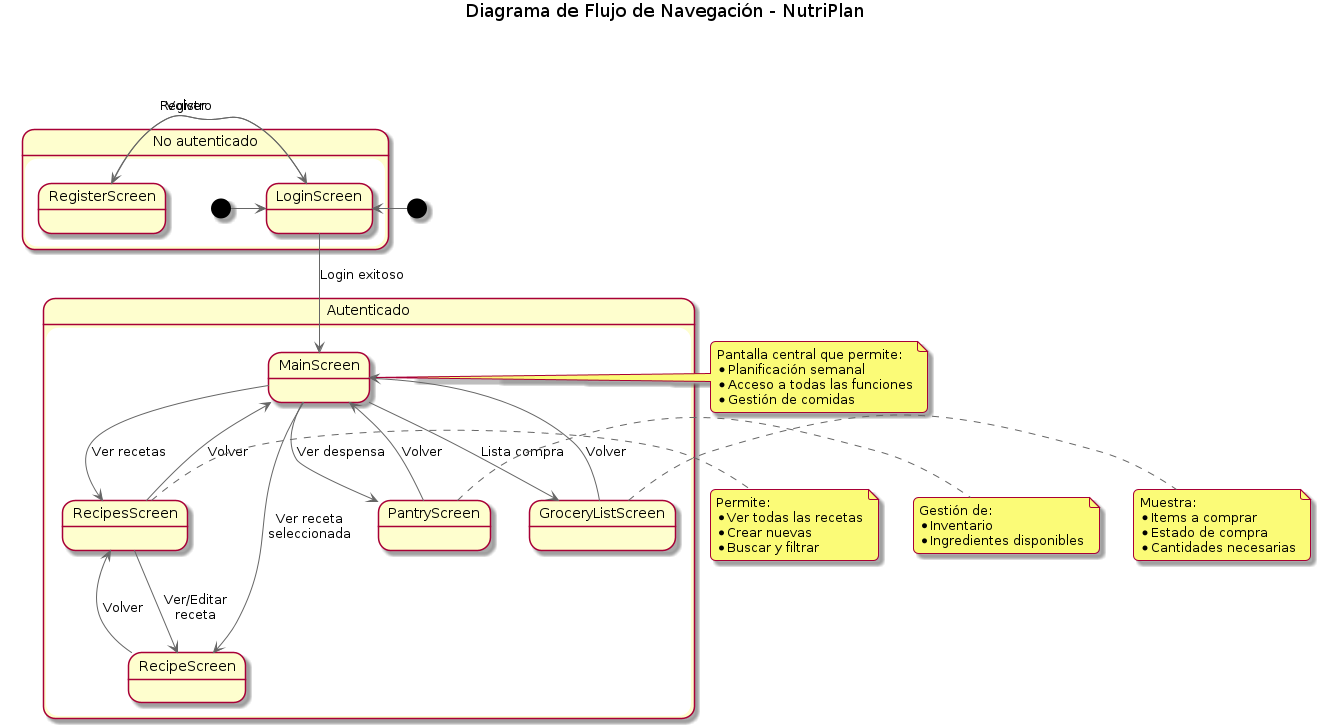
\includegraphics[width=\textwidth]{imagenes/navigation_flow}
			\caption{Diagrama de flujo de navegación de NutriPlan}
			\label{fig:navigation_flow}
		\end{figure}
		
		\subsubsection*{Organización y estructura visual}
		La interfaz se organizó priorizando la jerarquía visual y la facilidad de navegación:
		
		\begin{itemize}
			\item \textbf{Barra superior consistente:} Implementada en \texttt{AppHeader}, mantiene el contexto de navegación mostrando títulos en cada sección y provee acceso rápido a funciones y páginas principales. Esta decisión responde al principio de consistencia y reduce la carga cognitiva del usuario al mantener puntos de referencia estables.
			
			\item \textbf{Botones flotantes de acción:} El componente \texttt{FloatingButton} se utiliza para acciones principales (añadir receta, planificar comida) siguiendo patrones de Material Design. Su posición fija en la esquina inferior derecha facilita el acceso con el pulgar, mejorando la ergonomía en uso móvil.
			
			\item \textbf{Tarjetas y listas:} Los componentes \texttt{IngredientCard} y \texttt{RecipeCardComponent} presentan información en bloques visuales claramente delimitados, facilitando el escaneo rápido y la comprensión del contenido.
		\end{itemize}
		
		\subsubsection*{Paleta de colores}
		La selección de colores responde tanto a principios de accesibilidad como a la psicología del color en aplicaciones de alimentación:
		
		\begin{itemize}
			\item \textbf{Color primario:} Se eligieron como colores principales el blanco (\#FFF) y el naranja (\#FB7945). El blanco se utiliza principalmente para fondos de pantallas y de componentes; y los colores de las letras. El naranja se utiliza como color de fondo de los componentes(mayoritariamente botones) y también como color para resaltar elementos seleccionados.
			
			\item \textbf{Colores secundarios:} estos también son utilizados frecuentemente y son el gris claro (\#CCC) utilizado para separación sutil entre elementos, color de letras o como fondo de pantalla de otros. Los colores negro y blanco han sido usados para la letra.
			
		\end{itemize}
		
		Esta paleta no solo es estéticamente agradable sino que cumple con ratios de contraste WCAG 2.1 para garantizar accesibilidad.
		
		\subsubsection*{Interacción y feedback}
		El diseño de interacciones prioriza la eficiencia y claridad:
		
		\begin{itemize}
			
			\item \textbf{Gestos intuitivos:} Se implementaron gestos naturales como el mantener pulsado en un el \texttt{RecipeCard} para mostrar el modal de opciones
			
			\item \textbf{Feedback visual inmediato:} Cada acción (marcar ingrediente como comprado, añadir a la planificación) tiene una respuesta visual clara que confirma la operación.
		\end{itemize}
		
		\subsubsection*{Tipografía y legibilidad}
		Se utilizó una jerarquía tipográfica clara:
		
		\begin{itemize}
			\item \textbf{Títulos:} Fuente System Bold a 20pt para encabezados principales, garantizando visibilidad sin ser intrusiva.
			\item \textbf{Contenido:} System Regular a 16pt para el cuerpo, optimizando legibilidad en pantallas móviles.
			\item \textbf{Información secundaria:} System Light a 14pt para metadatos y detalles adicionales.
		\end{itemize}
		
		\subsubsection*{Adaptación a casos de uso}
		El diseño se alineó específicamente con los casos de uso principales:
		
		\begin{itemize}
			\item \textbf{Planificación semanal:} La vista principal (\texttt{MainScreen}) organiza la información por días y comidas, con un selector superior (\texttt{HeaderComponent}) que facilita la navegación temporal.
			
			\item \textbf{Gestión de recetas:} La interfaz de recetas prioriza imágenes y datos clave, permitiendo acceso rápido a ingredientes y cantidades mediante \texttt{IngredientComponent}.
			
			\item \textbf{Lista de compra:} \texttt{GroceryListScreen} implementa una visualización clara de items pendientes vs. comprados, con actualización inmediata del estado.
			
			\item \textbf{Control de despensa:} \texttt{PantryScreen} organiza ingredientes en categorías visuales claras, facilitando el inventario rápido.
		\end{itemize}
		
		\subsubsection*{Consideraciones de accesibilidad}
		El diseño incorpora elementos de accesibilidad básicos:
		
		\begin{itemize}
			\item Textos alternativos para imágenes
			\item Áreas táctiles generosas (mínimo 44x44 puntos)
			\item Contraste suficiente entre texto y fondo
			\item Soporte para el escalado de texto del sistema
		\end{itemize}
		
		\subsubsection*{Validación y mejoras futuras}
		El diseño actual establece una base sólida pero contempla evolución:
		
		\begin{itemize}
			\item Incorporación de temas oscuros para reducir fatiga visual
			\item Expansión de gestos y atajos para usuarios avanzados
			\item Mejora de la visualización de datos nutricionales
			\item Implementación de vistas adaptativas para tablets
		\end{itemize}
		
		Las decisiones de diseño tomadas buscan equilibrar simplicidad, eficiencia y satisfacción del usuario, creando una experiencia coherente que facilita la planificación alimentaria y reduce la fricción en tareas cotidianas. La adherencia a principios minimalistas y patrones establecidos de UX móvil contribuye a una curva de aprendizaje suave mientras se mantiene la potencia funcional necesaria.
	\section{Análisis de librerías y frameworks para el frontend y la lógica}
	En este apartado se explican qué son los frameworks y librerías más relevantes utilizados en el proyecto, se presentan las alternativas principales del mercado con sus ventajas e inconvenientes, y se justifica la elección final. Para facilitar la lectura se aborda con detalle React Native y Firebase (pues condicionan arquitectura y despliegue).
	
	\subsection{¿Qué es un framework / librería en este contexto?}
	En el ámbito del desarrollo móvil, un framework es un conjunto estructurado de herramientas, APIs y convenciones que facilita la creación de aplicaciones; una librería es un módulo reutilizable que proporciona funcionalidad concreta (UI, comunicación, almacenamiento, etc.). La elección de framework condiciona la arquitectura, el flujo de trabajo y las opciones de despliegue, mientras que la selección de librerías define aspectos concretos de la experiencia de desarrollo y del producto final.
	
	\subsection{React Native (análisis profundo)}
	React Native es un framework de código abierto propuesto por Meta que permite construir aplicaciones móviles utilizando JavaScript/TypeScript. A diferencia de enfoques híbridos que renderizan UI en un WebView, React Native mapea componentes declarativos a widgets nativos de cada plataforma.
	
	\paragraph{Alternativas principales}
	\begin{itemize}
		\item \textbf{Flutter (Google).} Framework que usa Dart y un motor propio de renderizado; dibuja toda la UI con su propia capa gráfica.
		\item \textbf{Desarrollo nativo (Kotlin/Java para Android, Swift/Objective‑C para iOS).} Máximo control y optimización, código específico por plataforma.
		\item \textbf{Soluciones híbridas (Ionic/Cordova, Capacitor).} Aplicaciones web empaquetadas con acceso a APIs nativas mediante puentes.
	\end{itemize}
	
	\paragraph{Ventajas y desventajas de cada alternativa}
	\begin{itemize}
		\item \textbf{React Native}
		\begin{itemize}
			\item Ventajas: reutilización de código entre plataformas, ecosistema maduro de librerías JS/TS, integración sencilla con módulos nativos, curva de entrada baja para desarrolladores web.
			\item Inconvenientes: en casos de UI muy compleja o rendimiento extremo puede requerir módulos nativos; la coordinación de versiones entre runtime y librerías exige mantenimiento.
		\end{itemize}
		
		\item \textbf{Flutter}
		\begin{itemize}
			\item Ventajas: rendimiento cercano a nativo; control total del rendering; experiencia UI homogénea entre plataformas.
			\item Inconvenientes: requiere aprender Dart y reescribir la UI; menor interoperabilidad directa con bibliotecas JS/TS del ecosistema web existente.
		\end{itemize}
		
		\item \textbf{Desarrollo nativo}
		\begin{itemize}
			\item Ventajas: máximo rendimiento y acceso completo a APIs; ideal para apps con requisitos muy específicos.
			\item Inconvenientes: doble esfuerzo de desarrollo y mantenimiento por plataforma; mayor coste y tiempo.
		\end{itemize}
		
		\item \textbf{Ionic / Cordova / Capacitor}
		\begin{itemize}
			\item Ventajas: desarrollo rápido con tecnologías web; buena opción para apps sencillas.
			\item Inconvenientes: limitaciones de rendimiento y experiencia nativa; comportamiento divergente en gestos y componentes nativos.
		\end{itemize}
	\end{itemize}
	
	\paragraph{Razones para elegir React Native en este proyecto}
	La elección de React Native responde a un equilibrio entre productividad y control técnico: permite desarrollar rápidamente con TypeScript, reutilizar lógica en toda la aplicación y aprovechar un amplio ecosistema (UI kits, navegación, integración con Firebase). Dado el alcance funcional de NutriPlan (formularios, listas, modales, acceso a cámara/galería y persistencia en la nube) React Native ofrece la combinación adecuada de eficiencia de desarrollo y capacidad para escalar con módulos nativos cuando sea necesario.

	\subsection{Otras librerías y componentes}
	
	
	\subsubsection*{Gestión de estado y contexto}
	Dada la complejidad de las aplicaciones y la variedad de componentes es complicado compartir datos entre distintas partes del programa. Un contexto se encarga de pasar información entre diferentes partes y niveles de una aplicación. Existen varias alternativas disponibles para esta función como:
	
	\begin{itemize}
		\item \textbf{React Context: } módulo de React que permite compartir funciones y estados entre componentes como si fueran variables globales. Es un componente nativo de React y no requiere de dependencias externas, fácil de añadir. Su único inconveniente es que afecta al rendimiento del software si no se planifica bien y no es compatible con estados o efectos complejos.
		\item \textbf{Redux: } librería de código abierto para el manejo de estados en JavaScript que permite mantener un estado globalizado en un componente llamado tienda (\textit{store}) y actualizarlo cuando sea necesario mediante las acciones guardadas en las funciones llamadas \textit{reducers}. Redux permite tener un estado predecible, escalable, fácil de depurar y consistente, pero al mismo tiempo no es un componente nativo de React, es complejo y por ende requiere experiencia y más código de lo usual para configuraciones básicas y excesivo para proyectos pequeños.
		\item \textbf{Zustand: } concepto similar a los anteriores solo que tiene una API muhco más simple que la de redux y un enfoque minimalista. Su simplicidad, flexibilidad, rapidez y no necesidad de \textit{wrappers} como \texttt{React Context} le hacen eficiente y fácil de utilizar.
	\end{itemize}

	Se ha usado \texttt{React Context} para el uso del contexto gracias a su facilidad de instalación, que se realiza en un sólo comando; su simplicidad y al tener una aplicación no tan compleja, esta librería no afectaría en el rendimiento.
	
	\subsubsection*{Navegación}
	La navegación en este caso es necesitada para la conexión entre pantallas permitiendo al usuario acceder a todo el contenido de la aplicación en un orden específico.  Existen varias alternativas como:
	
	\begin{itemize}
		\item \textbf{React Native Navigation}: librería creada por \textit{React Native} que permite la navegación e implementación de pilas (\textit{stack}), pestañas y bandejas de navegación, se integra con gestos y la navegación nativa de React Native, es fácil de utilizar, pero menos eficiente en grandes proyectos.
		\item \textbf{React Native Navigation(Wix)}: a diferencia de \textit{React Native Navigation} que usa JavaScript, esta usa las API nativas de navegación de iOS y Android, es más eficiente en grandes proyectos pero difícil de configurar.
	\end{itemize}
	
	Al estar trabajando en un proyecto simple que no requiere de muchas páginas ni tampoco utiliza pestañas o bandejas de navegación se ha utilizado \textit{React Native Navigation} para controlar las pantallas y su acceso dada su simplicidad de uso, fama y eficiencia en programas pequeños.
	
	\subsubsection*{\texttt{@rneui/themed} (React Native Elements) y UI kits}
	Conjunto de componentes de interfaz listos para usar (botones, inputs, cards, etc.).  
	Alternativas: React Native Paper, NativeBase, UI Kitten.  
	Ventajas: aceleración en la construcción de pantallas, tematización central, componentes coherentes. Inconvenientes: peso adicional en la app y limitaciones si se requiere personalización extrema.  
	Razón de elección: \texttt{@rneui/themed} proporciona los componentes que mejor encajan con el estilo requerido y permite personalizaciones sencillas sin reescribir elementos base; se usa en varios componentes del proyecto.
	
	\subsubsection*{Búsqueda local: \texttt{react-minisearch} (MiniSearch)}
	Motor de búsqueda en memoria ligero para texto indexa documentos y permite búsquedas por prefijo y ranking.  
	Alternativas: Fuse.js (búsqueda difusa), Lunr.js (índice invertido similar a motores más grandes).  
	Ventajas: MiniSearch es muy ligero, simple de integrar y suficiente para listas pequeñas/medianas como el catálogo de ingredientes. Inconvenientes: no diseñado para grandes volúmenes o búsqueda distribuida.  
	Por qué se escogió: en \texttt{IngredientSearchSelectorComponent} en la app se requiere latencia mínima y funcionamiento offline; MiniSearch satisface estos requisitos con bajo coste.
	
	\subsubsection*{Iconos: \texttt{react-native-vector-icons} (Ionicons)}
	Colección de iconos vectoriales para React Native con adaptadores para múltiples familias (Ionicons, Material, etc.).  
	Alternativas: usar SVGs con \texttt{react-native-svg}, o iconos del sistema.  
	Ventajas: fácil uso, consistencia visual y escalabilidad; amplia disponibilidad de glyphs. Inconvenientes: usado en cabeceras y botones.
	
	\subsubsection*{Pickers y selectores: \texttt{CustomPicker} y bibliotecas}
	Es un componente local \texttt{\hyperref[CustomPicker]{CustomPicker}} que abre un \texttt{Modal} con opciones para seleccionar el \texttt{quantityType}(unidad de métrica del ingrediente).
	Alternativas: \texttt{@react-native-picker/picker} (nativo) o \texttt{react-native-dropdown-picker} (más características).  
	Ventajas del enfoque actual: control total sobre la apariencia del modal y la interacción; comportamiento consistente en iOS/Android. Inconvenientes: requiere implementar accesibilidad y animaciones manualmente.  
	Razón de elección: necesidad de un comportamiento visual concreto integrado en \texttt{IngredientComponent} y de un control simple sobre apertura/cierre mediante las props \texttt{isPickerOpen} / \texttt{setIsPickerOpen}.
	
	
	
	\subsubsection*{Imágenes y selección de medios}
	Librería de gestión de imágenes mediante bibliotecas nativas (por ejemplo \texttt{react-native-image-picker}).  
	Alternativas: Expo Image Picker, soluciones servidoras.  
	Ventajas: acceso nativo a cámara/galería y control de permisos. Inconvenientes: configuración nativa inicial.  
	Razón: se eligió la solución que ofrece más control sobre permisos y procesado de imágenes en la ejecución nativa, no se puede utilizar la opción de \textit{Expo} ya que le proyecto no fué programado de manera nativa.
  
  
	\section{Análisis de librerías y frameworks para back-end}
		
		\subsection{Base de datos}
		Es el software encargado de guardar todos los datos necesarios del usuario y tenerlos al alcance en cualquier momento. Existen varias opciones que cubren nuestras necesidades, desde bases de datos locales hasta en la nube.
		\begin{itemize}
			\item \textbf{SQLite.} Es una base de datos relacional autónoma y ligera que es usada en proyectos locales y en línea; utiliza SQL como su lenguaje de programación, su instalación en \textit{React Native} es fácil e intuitiva. A pesar de que SQLite tiene esos beneficios, su integración en aplicaciones que necesitan bases de datos en la nube resulta complicado y costoso dado que SQLite no incorpora de forma nativa la sincronización de datos online.
			%
			\item \textbf{Firebase.} Plataforma creada por Google que integra servicios de autenticación, bases de datos en tiempo real, almacenamiento de ficheros, y herramientas auxiliares para análisis y despliegue. La mayor parte de sus servicios son gratuitos(hasta superar un límite establecido), a pesar de que su base de datos no sea relacional, no resulta difícil usarla como tal; su integración con \textit{React Native} se realiza en varios pasos y es muy simple; y por último tiene una comunidad muy grande que aporta documentación y \textit{feedback} extenso. En cuento a sus desventajas, estas son el no ser óptimo en relaciones o búsquedas complejas y su pago.
			%
			\item \textbf{SupaBase. } Base de datos de código abierto que utiliza 
			\textit{PostgreSQL} haciéndola muy robusta y potente, tiene atuenticación almacenamiento y funciones serverless(no requieren de servidor) y es gratuito gracias a su filosofía de código abierto. En cambio, no es tan maduro ni ampliamente probado en aplicaciones móviles (no tanto como Firebase), tiene una configuración e uso complejo y técnico y su documentación no es tan extensa.
			\item \textbf{MongoDb. } Base de datos local que contiene sincronización nativa con la nube, resulta óptima para aplicaciones que requieren de almacenamiento en y sin línea (online y offline) y el tipo de base de datos es similar al de \textit{Firebase}(no relacional). Sin embargo, su uso resulta complejo al añadir lógica personalizada al backend, no tiene una comunidad tan madura con React Native.
		\end{itemize}
	
		Para el backend se necesita una base de datos para una aplicación que no consume, no contiene muchos datos; que la base de datos sea minimalista en el aspecto del uso e instalación, pensada para app móviles y no tenga ningún coste económico. Firebase cumple con todas estas condiciones y además contiene servicios de autenticación y reglas de seguridad, por ello se escogió este como software de almacenamiento.
		
		
  	
	\section{Proyectos actuales}
	%Nombrar aplicaciones que hayan resultado de inspiración para el proyecto y explicar un poco de qué van esas aplicaciones
	  % ...existing code...
		\subsection*{Aplicaciones móviles existentes de meal planning}
		El interés creciente por planificar la alimentación doméstica ha dado lugar a aplicaciones con enfoques bien diferenciados: desde soluciones orientadas a la rapidez y conveniencia hasta plataformas centradas en el control nutricional o en la compra integrada. A continuación se exponen las diferencias esenciales entre las propuestas comerciales más conocidas y NutriPlan.
		
		\begin{itemize}
			\item \textit{\textbf{Mealime}} apuesta por la simplicidad y la velocidad: menús semanales preconfigurados y listas de compra automáticas reducen la fricción para el usuario que busca solucionar comidas sin preocuparse por detalles. Esa filosofía simplifica la adopción inicial pero sacrifica flexibilidad; las recetas y porciones estandarizadas limitan la capacidad de ajustar ingredientes, sustituir productos o conciliar con el inventario real del hogar. Para una herramienta cuyo valor diferencial es precisamente optimizar la lista de la compra en función de la despensa, esa pérdida de precisión es significativa.
			
			\item \textit{\textbf{Yazio}} sitúa el foco en el seguimiento nutricional: ofrecer conteo calórico y trazabilidad de macronutrientes requiere una base de datos nutricional rica y una interfaz que guíe al usuario en la introducción y el ajuste de datos. Es una excelente opción para objetivos de salud, pero su complejidad y el uso extendido de funciones premium añaden barreras de entrada. En el contexto de este proyecto, donde la prioridad es validar un flujo práctico (receta → planificación → despensa → lista) la profundidad nutricional extrema no aporta tanto valor inmediato como la fiabilidad en el cálculo de la compra y la experiencia off‑line.
			\item \textit{\textbf{Instacart}} se orienta hacia la transacción: conecta recetas y menús con la compra directa en supermercados asociados. Su fortaleza es la integración comercial y la comodidad para comprar en pocos pasos; su limitación es la dependencia de cobertura regional y acuerdos con comercios, además de que el objetivo principal es la venta más que la personalización dietética o la reducción del desperdicio.
		\end{itemize}
		  
		Frente a estos enfoques, NutriPlan se diseñó con prioridades claras y deliberadas: ofrecer control granular sobre las recetas, garantizar la conciliación precisa con la despensa del usuario, funcionar con baja latencia (incluso sin conexión) y mantener la propiedad y privacidad de los datos. Estas prioridades se tradujeron en decisiones técnicas y de producto concretas:
		
		\begin{itemize}
			\item \underline{Precisión y granularidad:} cada receta modela ingredientes con cantidad y unidad (\texttt{RecipeIngredient} en \texttt{src/Types/Types.tsx}), lo que permite cálculos exactos para la lista de la compra. Aunque exige mayor entrada de datos por parte del usuario, reduce el desperdicio y mejora la utilidad práctica del sistema.
			
			\item \underline{Disponibilidad y rendimiento:} la indexación local (MiniSearch) y la persistencia de Firestore proporcionan búsquedas instantáneas y operación offline para tareas frecuentes, mejorando la experiencia en contextos reales como tiendas con cobertura limitada.
			
			\item \underline{Privacidad y propiedad de datos:} los datos se aíslan por usuario (\texttt{uid}) y las reglas de seguridad de Firestore protegen la información personal; esta opción refuerza la confianza del usuario y facilita la portabilidad de los datos.
			
			\item \underline{Modelado equilibrado para BaaS:} el diseño de datos combina referencias y elementos embebidos para minimizar lecturas innecesarias en Firestore y mantener pantallas reactivas (p. ej. \texttt{MainScreen}, \texttt{GroceryListScreen}), reduciendo costes operativos y latencia.
			
			\item \underline{Onboarding progresivo y usabilidad:} la experiencia se organiza para que el usuario comience con tareas esenciales (añadir recetas, planificar, generar lista) y pueda acceder a funcionalidades más complejas solo si lo desea; la interfaz usa modales y componentes reutilizables (\texttt{src/Components/}) para minimizar el esfuerzo cognitivo.
			
			\item \underline{Modularidad y evolución:} la separación en capas (Components, Screens, Services, Context, Types) permite validar la idea con rapidez y mantener la puerta abierta a integraciones futuras (APIs de supermercados, motores de recomendación, o servicios avanzados de nutrición) sin reescribir la interfaz.
		\end{itemize}
		
			
			En conjunto, NutriPlan se sitúa entre las aplicaciones sencillas orientadas a la conveniencia y las plataformas complejas centradas en la nutrición o en el comercio electrónico. La elección de priorizar precisión en las recetas, conciliación con la despensa y operación offline responde a un objetivo práctico: reducir desperdicio y ofrecer una herramienta útil en el día a día del usuario. Estas decisiones, aunque aumentan la complejidad técnica inicial, maximizan el valor real entregado y facilitan evolucionar la aplicación hacia funcionalidades adicionales cuando la validación con usuarios lo aconseje.

	\section{Conclusiones}
	%Análisis propio (sin referencias bibliográficas) de lo que el autor considera sobre todo lo que ha explicado en el apartado de "Estado del arte". En nuestro caso, considerar qué librería es mejor que otra y en qué aspectos
	Tras analizar las distintas tecnologías y herramientas disponibles para el desarrollo de aplicaciones móviles, especialmente en el contexto de la planificación de comidas, podemos extraer conclusiones relevantes sobre las decisiones tomadas en este proyecto:
	
	\subsection*{Frameworks de desarrollo móvil}
	React Native ha demostrado ser la elección más adecuada frente a alternativas como Flutter o desarrollo nativo puro. Sus principales ventajas radican en:
	\begin{itemize}
		\item La capacidad de mantener una única base de código para iOS y Android, reduciendo significativamente el tiempo de desarrollo.
		\item Un ecosistema maduro de librerías que facilita la implementación de funcionalidades comunes.
		\item La posibilidad de aprovechar el conocimiento previo de JavaScript/TypeScript y React.
	\end{itemize}
	
	Sin embargo, es importante reconocer que Flutter podría ofrecer mejor rendimiento en aplicaciones con interfaces muy complejas o animaciones elaboradas. No obstante, para las necesidades de NutriPlan, donde prima la funcionalidad práctica sobre efectos visuales complejos, React Native proporciona el balance óptimo entre velocidad de desarrollo y rendimiento.
	
	\subsection*{Backend as a Service (BaaS)}
	Firebase ha resultado ser superior a alternativas como Supabase o un backend personalizado para este proyecto específico por:
	\begin{itemize}
		\item Facilidad de integración con React Native mediante SDKs oficiales.
		\item Capacidades de sincronización offline que mejoran la experiencia del usuario.
		\item Reducción significativa en tiempo de desarrollo al no requerir infraestructura propia.
	\end{itemize}
	
	Aunque las demás opciones ofrecen ventajas en términos de código abierto y control sobre los datos, Firebase proporciona una solución más madura y probada para las necesidades actuales de la aplicación. La decisión de usar Firestore sobre Realtime Database se justifica por su modelo de datos más flexible y mejor soporte para consultas complejas.
	
	\subsection*{Gestión de estado}
	La elección de React Context sobre alternativas como Redux o MobX se fundamenta en:
	\begin{itemize}
		\item Simplicidad en la implementación y menor curva de aprendizaje.
		\item Suficiente para la escala actual de la aplicación.
		\item Integración nativa con React sin dependencias adicionales.
	\end{itemize}
	
	Si bien Redux ofrece ventajas en aplicaciones más grandes, especialmente en términos de depuración y manejo de estados complejos, la sobrecarga que introduce no se justifica para el alcance actual de NutriPlan.
	
	\subsection*{Navegación y ruteo}
	React Navigation ha demostrado ser superior a alternativas como React Native Navigation (Wix) en nuestro caso por:
	\begin{itemize}
		\item API más intuitiva y documentación más completa.
		\item Mejor integración con el ecosistema React Native.
		\item Soporte nativo para gestos y animaciones en iOS y Android.
	\end{itemize}
	
	\subsection*{UI Components}
	La combinación de React Native Elements (@rneui/themed) con componentes personalizados ha resultado más efectiva que usar soluciones completas como Native Base o UI Kitten porque:
	\begin{itemize}
		\item Permite mayor flexibilidad en el diseño de la interfaz.
		\item Reduce el tamaño final de la aplicación al incluir solo los componentes necesarios.
		\item Facilita la personalización y consistencia visual.
	\end{itemize}
	
	\subsection*{Búsqueda y rendimiento}
	La implementación de búsqueda local con MiniSearch ha demostrado ser más eficiente que alternativas como Fuse.js o búsquedas en servidor por:
	\begin{itemize}
		\item Mejor rendimiento en búsquedas sobre conjuntos de datos medianos.
		\item Funcionamiento offline sin depender de la red.
		\item Menor consumo de recursos del dispositivo.
	\end{itemize}
	
	\subsection*{Conclusión general}
	Las decisiones tecnológicas tomadas priorizan tres aspectos fundamentales:
	\begin{enumerate}
		\item Velocidad de desarrollo y prototipado rápido.
		\item Experiencia de usuario fluida con buen rendimiento offline.
		\item Mantenibilidad y escalabilidad del código.
	\end{enumerate}
	
	Aunque existen alternativas que podrían ofrecer ventajas en aspectos específicos (rendimiento puro, control total sobre el backend, capacidades avanzadas de estado), las elecciones realizadas proporcionan el mejor compromiso para los objetivos del proyecto: crear una aplicación funcional, mantenible y con buena experiencia de usuario, permitiendo iteraciones rápidas y validación de funcionalidades con usuarios reales.

\chapter{Diseño y descripción del sistema}\label{cap.diseno y descripcion del sistema} %En este apartado se detallarían decisiones de diseño e implementación, como la decisión de utilizar React-Native y explicar por qué se ha elegido ese motor sobre otros
  \section{Mockups}
  %Explicar el diseño de la interfaz gráfica
  
  \section{Conclusiones}

\chapter{Prototipos y desarrollo}\label{cap.prototipos y desarrollo}
%Poner tantos prototipos como estimes necesario. En cada prototipo, meter alguna funcionalidad o completar alguna parte de la aplicación. Si mejoramos mucho algo, crear un prototipo nuevo.
  \section{Prototipo 1}
  \section{Prototipo 2}
  \section{Prototipo 3}
  \section{Conclusiones}

\chapter{Conclusiones y mejoras futuras}\label{cap.conclusiones y mejoras futuras}
  \section{Conclusiones técnicas}
  %Hablar desde el punto de vista del software de aspectos como el hecho de lo que nos ayuda React-Native
  \section{Conclusiones personales}
  %Valoración personal sobre cada una de las cosas vistas durante el proyecto
  \section{Futuras mejoras}
  %Trabajos futuros que se puedan relacionar con este

\chapter{Conclusions and future works}\label{cap.conclusions and future works}
  \section{Technical conclusions}
  \section{Personal conclusions}
  \section{Future works}

\cleardoublepage
\addcontentsline{toc}{chapter}{Bibliografía}
\bibliographystyle{acm} % estilo de la bibliografía.
\bibliography{citas} % citas.bib es el fichero donde está salvada la bibliografía.



\end{document}
